\chapter{Interpretazione astratta}
\section{Introduzione}
Nelle analisi precedenti l'approccio all'analisi statica è basato sull'informazione che
vogliamo osservare dell'esecuzione del programma, in particolare per proprietà relativamente semplici,
molto vicine alla sintassi che non descrivono informazioni sul contenuto delle variabili,
quindi in relazione agli elementi del programma piuttosto che al contenuto di tali elementi.

Per questo tipo di analisi, o in modo algoritmico fornendo direttamente l'equazione da risolvere, o 
in modo semantico, fornendo una semantica di elaborazione dell'informazione, costruita 
in modo induttivo sulla sintassi del linguaggio, riusciamo a fornire una soluzione sull'informazione
ricercata.

Il problema si pone quando vogliamo guardare ciò che accade al programma durante l'esecuzione, 
siamo quindi interessati a guardare all'interno delle stato della macchina, e non più alla relazione 
tra gli elementi del programma. Questo diventa relativamente un problema, poiché fornendo una 
semantica, tale semantica non risulterebbe distributiva, di conseguenza ci sarà necessariamente 
una perdita di informazione legata al fatto che risolvendo l'analisi localmente su punti di programma 
del \texttt{CFG} perdiamo informazione rispetto alla semantica desiderata, ovvero quella che considera 
tutti i cammini di esecuzione, ovvero la \textbf{MOP}. Si tratta del prezzo da pagare per rendere 
decidibile un calcolo su un informazione che si avvicina sempre di più all'informazione concreta, ovvero 
l'evoluzione dello stato della macchina.

Guardare all'interno dello stato della macchina significa avvicinarsi sempre di più 
all'informazione concreta, ma richiede un prezzo che è quello di staccarci 
dalla soluzione \textbf{MOP}, ottenendo attraverso la soluzione del calcolo 
di un sistema di disequazioni, una soluzione approssimata.

Nel momento in cui siamo interessati a guardare all'interno dello stato della macchina,
allora abbiamo bisogno, per mantenere delle garanzie sul calcolo della semantica astratta, 
di un'infrastruttura chiamata \textbf{interpretazione astratta}.

\begin{tcolorbox}[title=Interpretazione astratta]
    L'interpretazione astratta è un framework formale che permette di descrivere 
    dettagliatamente la relazione tra il momento concreto, di cui vogliamo dire 
    qualcosa, e il momento astratto, su cui possiamo dire qualcosa, garantendo informazioni 
    certe, anche se approssimate, su alcuni aspetti di interesse
    del mondo concreto.
\end{tcolorbox}
L'obiettivo è di verificare in modo automatico proprietà di interesse dei programmi e 
l'astrazione è il procedimento utilizzato per arginare il problema della non decidibilità
della semantica concreta.

\section{L'idea di base dell'interpretazione astratta}
L'idea di base è che un qualunque oggetto concreto sia formato da due elementi, un origine e 
un insieme finito di punti.

Supponiamo di definire nel nostro dominio concreto un oggetto fiore e vediamo come è possibile 
ottenerlo attraverso l'applicazione di operazioni concrete e partendo da operazioni concrete.
\begin{figure}[H]
    \centering 
    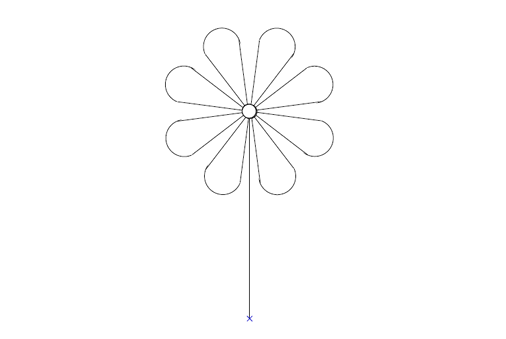
\includegraphics[scale=0.5]{img/flower.png}
\end{figure}
Tali oggetti non sono altro che dei numeri interni, quindi immaginiamo il fiore come una sequenza 
di operazioni che applichiamo ad elementi più piccoli, ovvero elementi del dominio stesso.
\subsection{Operazioni concrete}
Le operazioni che possiamo applicare sono le seguenti:
\begin{itemize}
    \item Costante: operazione che fornisce un petalo.
    \item Rotazione: $r[a](o)$ è un'operazione che ruota di $a$ gradi l'oggetto $o$.
    \begin{figure}[H]
        \centering 
        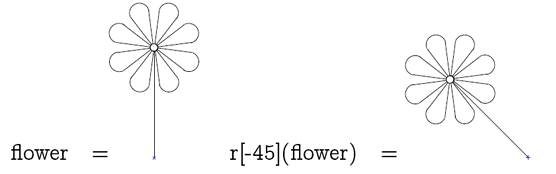
\includegraphics[scale=0.5]{img/rotation.png}
    \end{figure}
    \item Unione: $o_1 \cup o_2$ è un'operazione che unisce due oggetti $o_1$ e $o_2$, sovrapponendo 
    le origini.
    \begin{figure}[H]
        \centering 
        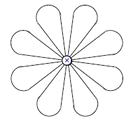
\includegraphics[scale=0.5]{img/corolla.png}
        \caption{$\texttt{corolla} = \texttt{petal} \cup r[45]\texttt{petal} 
        \cup r[90]\texttt{petal} \cup r[135]\texttt{petal}
        \cup r[180]\texttt{petal} \cup r[225]\texttt{petal} 
        \cup r[270]\texttt{petal} \cup r[315]\texttt{petal}$}
    \end{figure}
    \item \textit{stem}(o): è un'operazione che aggiunge un gambo all'oggetto $o$, il gambo viene sovrapposto 
    all'origine e la nuova origine è quella del gambo.
    \begin{figure}[H]
        \centering 
        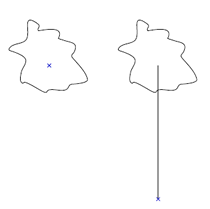
\includegraphics[scale=0.5]{img/stem.png}
    \end{figure}
\end{itemize}
Per la costruzione della corolla possiamo trovare un operatore monotono che applicato iterativamente 
fino al raggiungimento di un punto fisso, ci permette di ottenere la corolla. Possiamo costruire oggetti 
concreti per punto fisso a partire da oggetti più semplici, che è ciò che avviene con la semantica.
\[
  \texttt{corolla} = lfp^{\subseteq} F  
\]
\[
    F(X) = \texttt{petal} \cup r[45](X)
\]
\begin{figure}[H]
    \centering
    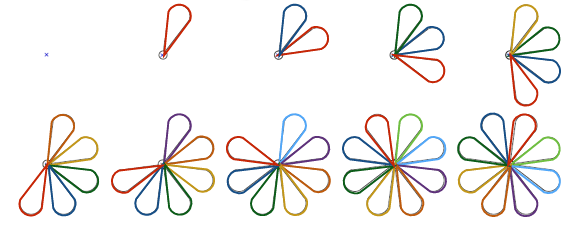
\includegraphics[scale=0.5]{img/fixpointcorolla.png}
\end{figure}
Abbiamo quindi introdotto un dominio concreto di oggetti su cui abbiamo definito delle operazioni.
\subsection{Approssimazione verso l'alto}
Operare su tali oggetti può comportare situazioni di non decidibilità, l'idea è quindi di approssimare 
tali oggetti concreti.
Definiamo la relazione di approssimazione, ovvero cosa vuol dire essere meno precisi. Nel caso degli 
oggetti, quello che è essere meno precisi è avere la stessa origine, ma che contengono più pixel, ovvero 
aggiungere rumore rispetto all'informazione originale.
\begin{figure}[H]
    \centering
    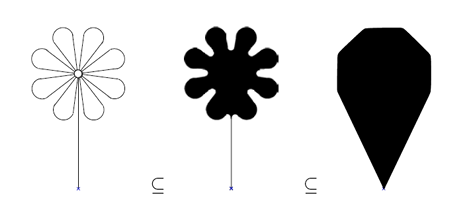
\includegraphics[scale=0.5]{img/upperapprox.png}
\end{figure}
In questo particolare caso abbiamo perso parte del dettaglio della figura, in particolare la corolla.
Aver più pixel aggiunge quindi rumore.

\subsection{Oggetti astratti}
L'oggetto astratto è una rappresentazione di un oggetto concreto che vogliamo fornire in 
forma approssimata. Decidiamo di rappresentare l'insieme di pixel dal suo contorno.
Questo è l'ordine che inseriamo nel dominio di computazione, propagando l'ordinamento,
che nel dominio concreto è dato dal contenimento, sul dominio astratto.
Un oggetto è quindi più astratto se è la rappresentazione di un oggetto concreto più grande.
\begin{figure}[H]
    \centering
    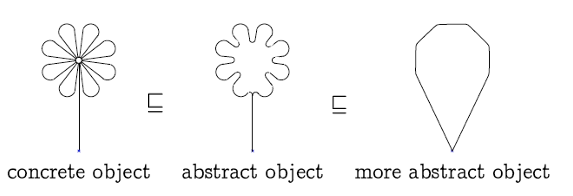
\includegraphics[scale=0.6]{img/abstractobj.png}
\end{figure}
L'idea è che il contorno di un certo oggetto venga disegnato con una pennarello 
di spessore variabile, la variabilità di tale spessore è data dal livello di astrazione.
Disegnando un un pennarello più spesso, si perde dettaglio, mentre disegnando
con un pennarello più sottile, si guadagna dettaglio.

\begin{tcolorbox}[title = Dominio astratto]
    Il dominio astratto è l'insieme di tutti gli oggetti astratti, più 
    le operazioni astratte che permettono di costruire oggetti astratti
    (\textit{che approssimano le operazioni concrete}).
\end{tcolorbox}
\begin{tcolorbox}[title =  Astrazione]
    L'astrazione è una funzione $\alpha$ che mappa ogni oggetto concreto
    in una approssimazione rappresentata da un oggetto astratto $\alpha(o)$
    in modo univoco.
\end{tcolorbox}
Il tutto è costruito in modo tale da poter confrontare oggetti astratti 
tra di loro, scegliendo di guardare l'informazione approssimata allargando 
il diametro del pennarello.
\subsection{Concretizzazione}
Nel mondo dell'interpretazione astratta corrisponde ad assegnare il significato 
concreto dell'oggetto astratto che stiamo osservando.

Nel caso degli oggetti rappresentati precedentemente, la concretizzazione
è possibile vederla come l'idea di riempire il contorno dell'oggetto astratto.
\begin{figure}[H]
    \centering
    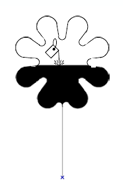
\includegraphics[scale=0.6]{img/concretizzazione.png}
\end{figure}
Si tratta di una funzione $\gamma$ che mappa ogni oggetto
astratto $\bar{o}$ in un oggetto concreto, in modo univoco
$\gamma(\bar{o})$.

Prendendo in considerazione l'insieme $\{2,6\}$ l'astrazione
di tale insieme, ovvero l'applicazione $\alpha$, può essere visto come la 
funzione che mappa l'insieme $\{2,6\}$ (\textit{fiore concreto}) in un oggetto astratto
che rappresenta l'insieme $2\mathbb{Z}$ (\textit{fiore astratto}). L'applicazione 
della funzione $\gamma$ su tale oggetto astratto, fa si che 
si ottenga $\{0,2,4,6,\dots\}$ (\textit{fiore riempito}).
\subsection{Connessione di Galois}
Queste due funzioni di concretizzazione e astrazione nell'interpretazione
astratta sono modellate dal concetto di \textbf{connessione di Galois}.

Dice infatti che è una coppia di funzioni, tali che:
\begin{itemize}
    \item $\alpha$ è monotona
    \begin{figure}[H]
        \centering
        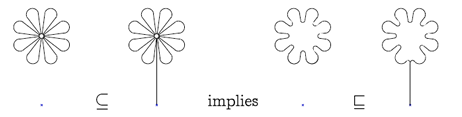
\includegraphics[scale=0.6]{img/galoisconn1.png}
    \end{figure}
    \item $\gamma$ è monotona
    \begin{figure}[H]
        \centering
        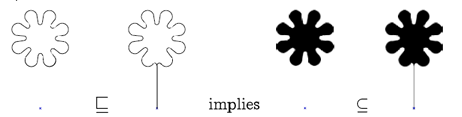
\includegraphics[scale=0.6]{img/galoisconn2.png}
    \end{figure}
\end{itemize}
La monotonia fa si che preservino l'ordine tra i due domini.

In più le connessioni di Galois devono estendere quando si esegue 
il processo di astrazione, quindi il processo di astrazione può aggiungere 
rumore:
\[
    \textit{per ogni oggetto concreto } x, \gamma \circ \alpha(x) \subseteq x
\]
\begin{figure}[H]
    \centering
    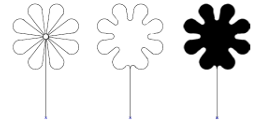
\includegraphics[scale=0.6]{img/galoisconn3.png}
\end{figure}
Inoltre se prima concretizziamo e poi astraiamo, otteniamo
un oggetto astratto più piccolo di quello di partenza, questo perché 
nel mondo concreto potrebbero esserci oggetti inutili che non hanno significato.
\[
    \textit{per ogni oggetto astratto } y, \alpha \circ \gamma(y) \sqsubseteq  y
\]
Tipicamente si ha che $\alpha \circ \gamma(y) = y$.
\begin{figure}[H]
    \centering
    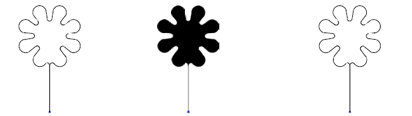
\includegraphics[scale=0.6]{img/galoisconn4.png}
\end{figure}
\subsection{Ordinamento astratto}
L'ordinamento astratto è il trasferimento dell'ordinamento concreto
sul dominio astratto. Quindi un oggetto astratto è più piccolo di un altro
oggetto astratto se la corrisponde concretizzazione è più piccola.
\begin{figure}[H]
    \centering
    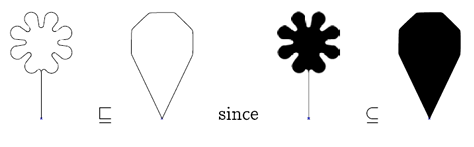
\includegraphics[scale=0.6]{img/abstractordering.png}
\end{figure}
In origine ciò che volevamo fare era calcolare delle operazioni sul dominio concreto 
con l'assunzione che tali operazioni non fossero sempre decidibili. L'obiettivo 
è trasferire tali operazioni dal mondo concreto al mondo astratto, in modo tale
da poterle calcolare in modo sempre decidibile.
Il modo più immediato per farlo è quello di passare attraverso le operazioni concrete.
Nell'esempio del gambo abbiamo in fatti che:
\[
    \overline{\texttt{stem}} = \alpha (\texttt{stem} (\gamma(y)))
\]
\begin{figure}[H]
    \centering
    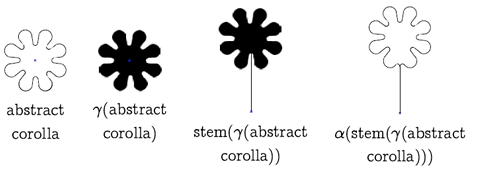
\includegraphics[scale=0.6]{img/abstractstem.png}
\end{figure}
Non potevamo aggiungere direttamente il gambo alla corolla astratta 
poiché avremmo avuto un livello di dettaglio diverso dal risultato finale 
che non avrebbe coinciso con lo spessore del pennarello scelto per 
osservare l'oggetto concreto.
È necessario definire un'operazione ad hoc per
poter lavorare su oggetti astratti, preservando quindi l'informazione che 
abbiamo sull'oggetto astratto, ovvero che il suo contorno è stato delimitato 
con un certo spessore e su tutte le operazioni è possibile eseguire 
tale passaggio.
\subsection{Punto fisso astratto}
Esattamente come le operazioni precedenti, anche il calcolo di punto fisso 
può essere trasferito dal mondo concreto a quello astratto.

Possiamo eseguire direttamente un'astrazione del punto fisso:
\[
  \texttt{abstract corolla} = \alpha(\texttt{concrete corolla}) =
    \alpha(lfp^{\subseteq} F)  
\]
Dove $F(X)= \texttt{petal} \cup r[45](X)$.
Sappiamo però che possa ereditare problemi di decidibilità 
e di convergenza, poiché il punto fisso se esiste in presenza di 
funzioni monotone, può divergere. È chiaro che poiché ci spostiamo 
nel mondo astratto per controllare questo tipo di divergenza, non avrebbe 
senso calcolare il punto fisso concreto e poi astrarlo. L'obiettivo 
è quello di costruire un operatore astratto il cui punto fisso nel mondo 
ideale che sia esattamente l'astrazione del punto fisso concreto, 
però con il fatto il punto fisso astratto è calcolato su un mondo 
approssimato e quindi potenzialmente convergente.
\[
    \alpha(lfp^{\subseteq} F) = lfp^{\sqsubseteq} \overline{F}
\]
In generale si tratta della situazione ideale, in cui abbiamo costruito 
esattamente l'operatore di punto fisso che sul nostro dominio riesce 
a raggiungere precisamente la proprietà del punto fisso concreto.
In generale quello che succede è che il punto fisso astratto sarà 
un'approssimazione ulteriore della proprietà del punto fisso concreto.

\begin{figure}[H]
    \centering
    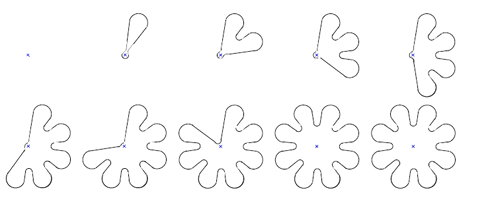
\includegraphics[scale=0.6]{img/abstractfixpoint.png}
\end{figure}

\section{Costruzione formale dell'interpretazione astratta}
Vediamo ora gli strumenti formali che utilizziamo per modellare e 
descrivere quelle che sono le basi dell'interpretazione astratta.

Il concetto principale utilizzato per descrivere l'interpretazione astratta,
ovvero il legame che c'è tra mondo concreto, nel quale vogliamo calcolare una 
semantica e nel quale vorremmo dare risposte, e il mondo astratto,
nel quale potenzialmente possiamo calcolare la semantica, e nel quale possiamo 
dare delle risposte, sono le \textbf{connessioni di Galois}.
Per farlo dobbiamo costruire questo mondo astratto nel rispetto di 
alcuni vincoli, in modo tale da dare determinate garanzie sul passaggio dal mondo 
concreto al mondo astratto.

Non si tratta dell'unico strumento formale, ma alcuni di questi sono 
completamente equivalenti.

\begin{tcolorbox}[title = Connessione di Galois]
    La connessione di Galois \texttt{GC} è una coppia di funzioni monotone 
    $\alpha$ e $\gamma$ definite tra un dominio concreto $\mathcal{C}$ e un dominio
    astratto $\mathcal{A}$.
\end{tcolorbox}
In generale $\mathcal{A}$ e $\mathcal{C}$ possono essere dei \textit{poset}, per semplicità di 
formalizzazione consideriamo $\mathcal{A}$ e $\mathcal{C}$ come reticoli completi, dove è quindi 
definito un \textit{least upper bound} e un \textit{greatest lower bound}, oltre 
all'ordine parziale. Gli ordinamenti sono definiti come segue:
\begin{itemize}
    \item $(\mathcal{A}, \leq)$;
    \item $(\mathcal{C}, \leq)$;
\end{itemize}

Le due funzioni sono definite come segue:
\begin{itemize}
    \item $\alpha: \mathcal{C} \rightarrow \mathcal{A}$ è detta di \textbf{astrazione}
    \item $\gamma: \mathcal{A} \rightarrow \mathcal{C}$ è detta di \textbf{concretizzazione}
\end{itemize}
$\alpha$ e $\gamma$ formano una connessione di Galois se sono monotone, ovvero: 
\[
    \forall x, y \in \mathcal{C} . x \leq_\mathcal{C} y \implies \alpha(x) \leq_\mathcal{A} \alpha(y)
\]
\[
    \forall x, y \in \mathcal{A} . x \leq_\mathcal{A} y \implies \gamma(x) \leq_\mathcal{C} \gamma(y)
\]
e $\alpha(c) \leq_\mathcal{A} a \iff c \leq_\mathcal{C} \gamma(a)$.

\begin{figure}[H]
    \centering
    \begin{tikzpicture}[>=stealth, node distance=2cm]

        % Define styles
        \tikzstyle{set} = [ellipse, draw, minimum height=4cm, minimum width=6cm, align=center]
        \tikzstyle{arrow} = [->, thick];
    
        % Nodes
        \node[set] (C) at (0,0) {$C$};
        \node[set, right=of C] (A) {$A$};
        
        
        \node[circle, draw, fill=black, inner sep=2pt, label=below:$c$] (pointC) at (1,-1) {};
        \node[circle, draw, fill=black, inner sep=2pt, label=below:$\alpha(c)$] (pointAlphaC) at (7,-1) {};
        \draw[arrow, orange] (pointC) to [bend left] (pointAlphaC);
        \node[circle, draw, fill=black, inner sep=2pt, label=above:$a$] (pointA) at (7,0) {};
        \draw[-, thick] (pointAlphaC) to (pointA);
        \node[circle, draw, fill=black, inner sep=2pt, label=above:$\gamma(a)$] (pointGammaA) at (1,0) {};
        \draw[arrow, green] (pointA) to [bend right] (pointGammaA);
        \draw[-, thick] (pointGammaA) to (pointC);

        % Scrivo alpha sopra la freccia
        \node at (4,0.2) {$\alpha$};
        \node at (4,1.2) {$\gamma$};
        
    \end{tikzpicture}
\end{figure}
Dire che l'astrazione di un elemento è più piccolo di un certo oggetto 
astratto equivale a dire che la concretizzazione di tale oggetto astratto 
è più grande dell'oggetto astratto da cui siamo partiti.

In generale $\alpha$ è chiamata aggiunta a destra,
mentre $\gamma$ è chiamata aggiunta a sinistra.

La monotonia garantisce di preservare l'ordine, mentre la condizione 
$\alpha(c) \leq_\mathcal{A} a \iff c \leq_\mathcal{C} \gamma(a)$ garantisce l'esistenza,
nel mondo astratto, della migliore approssimazione possibile per 
ogni elemento concreto.

Come notazione, la connessione di Galois è rappresentata
come segue: 
\[(\mathcal{C}, \leq_\mathcal{C}) \galois{\alpha}{\gamma} (\mathcal{A}, \leq_\mathcal{A})\]
Inoltre la condizione $\alpha(c) \leq_A a \iff c \leq_C \gamma(a)$
equivale a dire che:
\[c \leq_\mathcal{C} \gamma \, \circ \, a(c) \iff \alpha \, \circ \, \gamma(a) \leq_\mathcal{A} a\]
questo perché non ponendo vincoli sul dominio astratto, può essere che 
vi siano elementi assolutamente inutili per rappresentare la proprietà
che ci interessa osservare e tali elementi hanno un significato che coincide al significato di 
altri elementi astratti. Avendo più elementi astratti con lo stesso significato e supponendo che 
$a$ abbia lo stesso significato di $\alpha(c)$, applicando la funzione $\gamma$ entrambi gli elementi 
vengono mappati sullo stesso elemento concreto, e tornando indietro con $\alpha$ si ottiene
si ottiene $\alpha(c)$.

Le inserzioni di Galois, invece, differiscono dalle connessioni di Galois nel fatto che 
$c \leq_\mathcal{C} \gamma \, \circ \, a(c)$ diventa un'uguaglianza, quindi:
\[c \leq_\mathcal{C} \gamma \, \circ \, a(c) \iff \alpha \, \circ \, \gamma(a) = a\]
Hanno come caratteristica di non avere nel dominio astratto $A$ nessun elemento inutile, 
quindi ogni elemento astratto ha uno specifico significato concreto che ci interessa 
osservare. Catturano meglio perché catturano tutti gli elementi significativi del dominio.

La rappresentazione dell'inserzione di Galois è la seguente:
\[(\mathcal{C}, \leq_\mathcal{C}) \galoiS{\alpha}{\gamma} (\mathcal{A}, \leq_\mathcal{A})\]
Poiché $\alpha$ è una funzione suriettiva.

Ogni connessione di Galois può essere ridotta ad una inserzione di Galois, eliminando 
gli elementi astratti inutili, ovvero quelli per cui esiste un elemento più piccolo che 
ha lo stesso significato.
\subsection{Esempio di inserzione e connessione di Galois}
Vogliamo vedere cosa vuol dire quando abbiamo a disposizione una connessione di Galois 
che non è effettivamente un'inserzione di Galois, con elementi inutili nel nostro 
dominio astratto, ridurre la connessione di Galois ad una inserzione di Galois.

Supponiamo di disporre di questi due domini, dove il dominio concreto è 
$\wp(\mathcal{A})$ e come dominio astratto abbiamo $\wp(\mathcal{B})^d$, dove 
$\wp(\mathcal{B})^d$ è ordinato per inclusione inversa.

\begin{figure}[H]
    \centering
    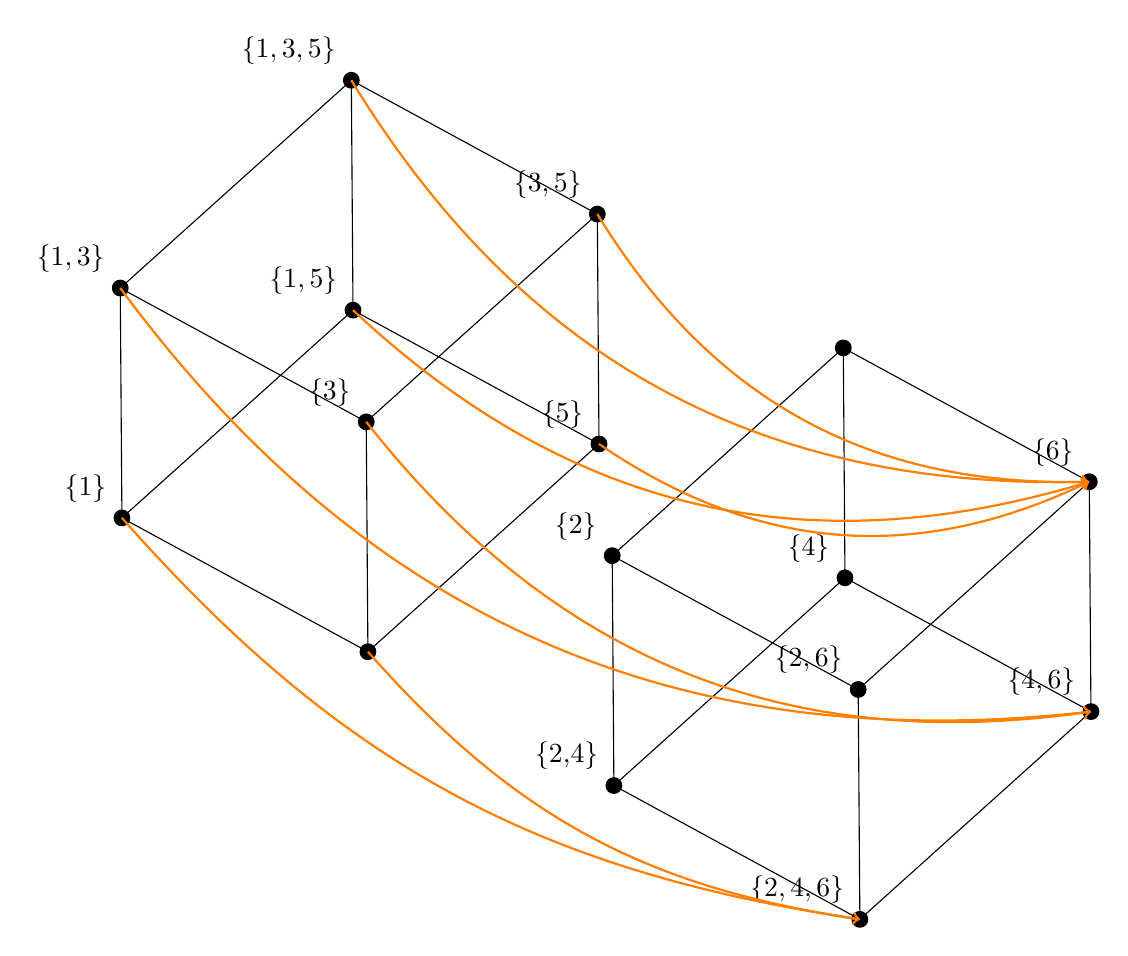
\begin{tikzpicture}[transform shape, rotate around z=-10, rotate around x=25, rotate around y=-20]

        \coordinate (A) at (0,0,0);
        \coordinate (B) at (4,0,0);
        \coordinate (C) at (4,4,0);
        \coordinate (D) at (0,4,0);
        \coordinate (E) at (0,0,4);
        \coordinate (F) at (4,0,4);
        \coordinate (G) at (4,4,4);
        \coordinate (H) at (0,4,4);

        \foreach \p/\t in { A/{$\{1,5\}$},
                            B/{$\{5\}$},
                            C/{$\{3,5\}$},
                            D/{$\{1,3,5\}$},
                            E/{\{1\}},
                            F/{$\varnothing$},
                            G/{$\{3\}$},
                            H/{$\{1,3\}$}}
            \node[draw, fill, circle, inner sep=2pt, label={135:\t}] (A\p) at (\p) {};

        \draw (A) -- (B) -- (C) -- (D) -- cycle; % Base
        \draw (E) -- (F) -- (G) -- (H) -- cycle; % Top
        \draw (A) -- (E);
        \draw (B) -- (F);
        \draw (C) -- (G);
        \draw (D) -- (H);

        \coordinate (I) at (8,0,0);
        \coordinate (J) at (12,0,0);
        \coordinate (K) at (12,4,0);
        \coordinate (L) at (8,4,0);
        \coordinate (M) at (8,0,4);
        \coordinate (N) at (12,0,4);
        \coordinate (O) at (12,4,4);
        \coordinate (P) at (8,4,4);

        \foreach \p/\t in { I/{$\{4\}$},
                            J/{$\{4,6\}$},
                            K/{$\{6\}$},
                            L/{$\varnothing$},
                            M/{\{2,4\}},
                            N/{$\{2,4,6\}$},
                            O/{$\{2,6\}$},
                            P/{$\{2\}$}}
            \node[draw, fill, circle, inner sep=2pt, label={135:\t}] (B\p) at (\p) {};

        \draw (I) -- (J) -- (K) -- (L) -- cycle; % Base
        \draw (M) -- (N) -- (O) -- (P) -- cycle; % Top
        \draw (I) -- (M);
        \draw (J) -- (N);
        \draw (K) -- (O);
        \draw (L) -- (P);

        \draw[->, color=orange, bend right=20, thick] (E) to node[above] {} (N);
        \draw[->, color=orange, bend right=20, thick] (F) to node[above] {} (N);
        \draw[->, color=orange, bend right=30, thick] (G) to node[above] {} (J);
        \draw[->, color=orange, bend right=30, thick] (H) to node[above] {} (J);
        \draw[->, color=orange, bend right=30, thick] (A) to node[above] {} (K);
        \draw[->, color=orange, bend right=30, thick] (B) to node[above] {} (K);
        \draw[->, color=orange, bend right=30, thick] (C) to node[above] {} (K);
        \draw[->, color=orange, bend right=30, thick] (D) to node[above] {} (K);
    \end{tikzpicture}
\end{figure}
L'obiettivo è costruire una funzione di concretizzazione che permetta di 
vedere l'insieme a destra come un'astrazione del dominio a sinistra.
\[
  \forall \mathcal{A}' \subseteq \mathcal{A} .
  \quad \alpha(\mathcal{A}') = \{b \in \mathcal{B} \mid \mathcal{A}' \subseteq b\}  
\]
Dove dal punto di vista formale si tratta di una funzione monotona che 
mappa un insieme nell'insieme più grande di 
elementi in cui tutti gli elementi sono più grandi dell'insieme di partenza.

Da quello che osserviamo solo tre elementi di elementi sono immagine di 
$\alpha$ secondo la definizione.

Tutti gli altri elementi sono inutili all'interno del significato di 
tale astrazione. Fatto che possiamo verificare calcolando la funzione 
$\gamma$ che è la funzione di astrazione.
\[
  \forall \mathcal{B}' \subseteq \mathcal{B} . 
    \quad \gamma(\mathcal{B}') = \{ a \in \mathcal{A} \mid a \subseteq \mathcal{B}' \}
\]
La funzione $\gamma$ preso un elemento astratto restituisce il suo significato 
concreto, in questo caso l'insieme massimale di elementi che sono più piccoli.
\begin{figure}[H]
    \centering
    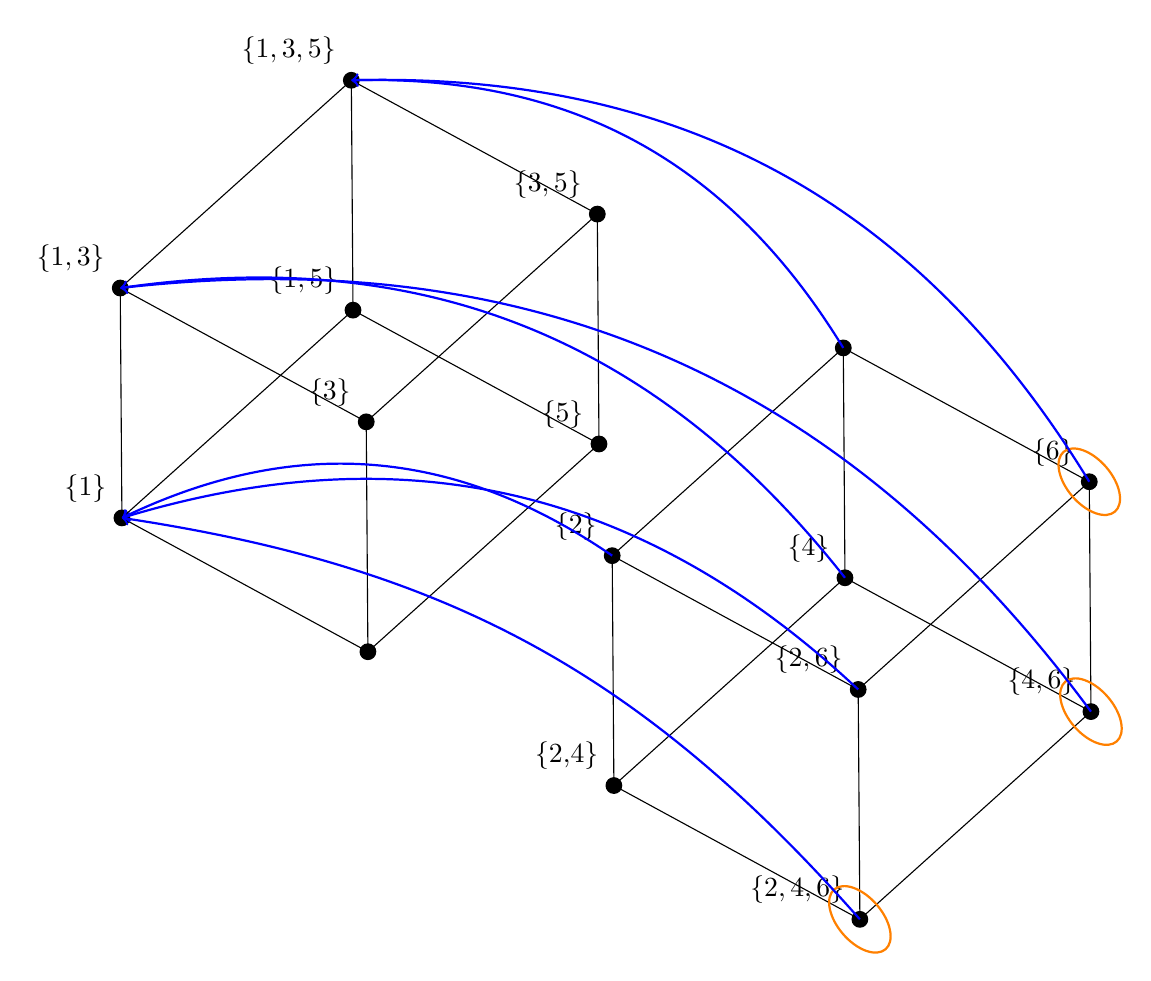
\begin{tikzpicture}[transform shape, rotate around z=-10, rotate around x=25, rotate around y=-20]

        \coordinate (A) at (0,0,0);
        \coordinate (B) at (4,0,0);
        \coordinate (C) at (4,4,0);
        \coordinate (D) at (0,4,0);
        \coordinate (E) at (0,0,4);
        \coordinate (F) at (4,0,4);
        \coordinate (G) at (4,4,4);
        \coordinate (H) at (0,4,4);

        \foreach \p/\t in { A/{$\{1,5\}$},
                            B/{$\{5\}$},
                            C/{$\{3,5\}$},
                            D/{$\{1,3,5\}$},
                            E/{\{1\}},
                            F/{$\varnothing$},
                            G/{$\{3\}$},
                            H/{$\{1,3\}$}}
            \node[draw, fill, circle, inner sep=2pt, label={135:\t}] (A\p) at (\p) {};

        \draw (A) -- (B) -- (C) -- (D) -- cycle; % Base
        \draw (E) -- (F) -- (G) -- (H) -- cycle; % Top
        \draw (A) -- (E);
        \draw (B) -- (F);
        \draw (C) -- (G);
        \draw (D) -- (H);

        \coordinate (I) at (8,0,0);
        \coordinate (J) at (12,0,0);
        \coordinate (K) at (12,4,0);
        \coordinate (L) at (8,4,0);
        \coordinate (M) at (8,0,4);
        \coordinate (N) at (12,0,4);
        \coordinate (O) at (12,4,4);
        \coordinate (P) at (8,4,4);

        \foreach \p/\t in { I/{$\{4\}$},
                            J/{$\{4,6\}$},
                            K/{$\{6\}$},
                            L/{$\varnothing$},
                            M/{\{2,4\}},
                            N/{$\{2,4,6\}$},
                            O/{$\{2,6\}$},
                            P/{$\{2\}$}}
            \node[draw, fill, circle, inner sep=2pt, label={135:\t}] (B\p) at (\p) {};

        \draw (I) -- (J) -- (K) -- (L) -- cycle; % Base
        \draw (M) -- (N) -- (O) -- (P) -- cycle; % Top
        \draw (I) -- (M);
        \draw (J) -- (N);
        \draw (K) -- (O);
        \draw (L) -- (P);

        %cerchio i punti che sono immagine di alpha
        \draw[circle, color=orange, thick] (K) circle (0.5);
        \draw[circle, color=orange, thick] (J) circle (0.5);
        \draw[circle, color=orange, thick] (N) circle (0.5);

        \draw[->, color=blue, bend right=20, thick] (N) to node[above] {} (E);
        \draw[->, color=blue, bend right=30, thick] (O) to node[above] {} (E);
        \draw[->, color=blue, bend right=30, thick] (P) to node[above] {} (E);
        \draw[->, color=blue, bend right=30, thick] (J) to node[above] {} (H);
        \draw[->, color=blue, bend right=30, thick] (I) to node[above] {} (H);
        \draw[->, color=blue, bend right=30, thick] (K) to node[above] {} (D);
        \draw[->, color=blue, bend right=30, thick] (L) to node[above] {} (D);
\end{tikzpicture}
\end{figure}
Quindi emergono 3 elementi, ovvero $\{1,3,5\}$, $\{1,3\}$ e $\{1\}$,
che sono i più concreti tra quelli che hanno la stessa 
immagine astratta, ovvero $\{4\}$, $\{4,6\}$ e $\{6\}$.

Verifichiamo che $\alpha$ e $\gamma$ rispettano le condizioni sull'essere 
connessioni di Galois.

Partendo dall'insieme vuoto e applicando $\alpha$ otteniamo l'insieme
$\{4\}$ che è l'immagine astratta di $\{ 2,4,6 \}$, applicando $\gamma$
otteniamo l'insieme $\{1\}$. Quindi
$\gamma \circ \alpha(\varnothing) \geq \varnothing$, e provandolo per tutti 
gli elementi otteniamo lo stesso risultato generico:
\[
  \gamma \circ \alpha(c) \geq c  
\]
e anche la condizione opposta:
\[
  \alpha \circ \gamma(a) \leq a
\]
Quindi $\alpha$ e $\gamma$ sono connessioni di Galois.

Per riuscire a eliminare gli elementi inutili possiamo applicare
il concetto relativo all'inserzione di Galois, quindi:
\[
  \mathcal{B}' \equiv \mathcal{B}''
  \iff \gamma(\mathcal{B}') = \gamma(\mathcal{B}'') 
  \iff \forall a \in
  \mathcal{A} . \quad a \mathcal{RB}' \iff a \mathcal{RB}'' 
\]
La differenza è che $ \alpha \circ \gamma(a) = a $, quindi
vediamo che modificando il dominio astratto e non le astrazioni 
otteniamo un'inserzione di Galois, osserviamo quindi gli elementi che 
hanno lo stesso significato.
quindi:
\begin{itemize}
    \item $\varnothing$ e $\{6\}$ hanno lo stesso significato, quindi
    vengono mappati in un unico elemento, che è $\{6\}$;
    \item $\{4\}$ e $\{4,6\}$ hanno lo stesso significato, quindi
    vengono mappati in un unico elemento, che è $\{4,6\}$;
    \item $\{2,4\}$, $\{2,4,6\}$, $\{2,6\}$ e $\{2\}$ hanno lo stesso
    significato e vengono mappati in un unico elemento, che è $\{2,4,6\}$.
\end{itemize} 
Accorpando gli elementi astratti che hanno lo stesso significato.
Quindi otteniamo il seguente diagramma:
\begin{figure}[H]
    \centering
    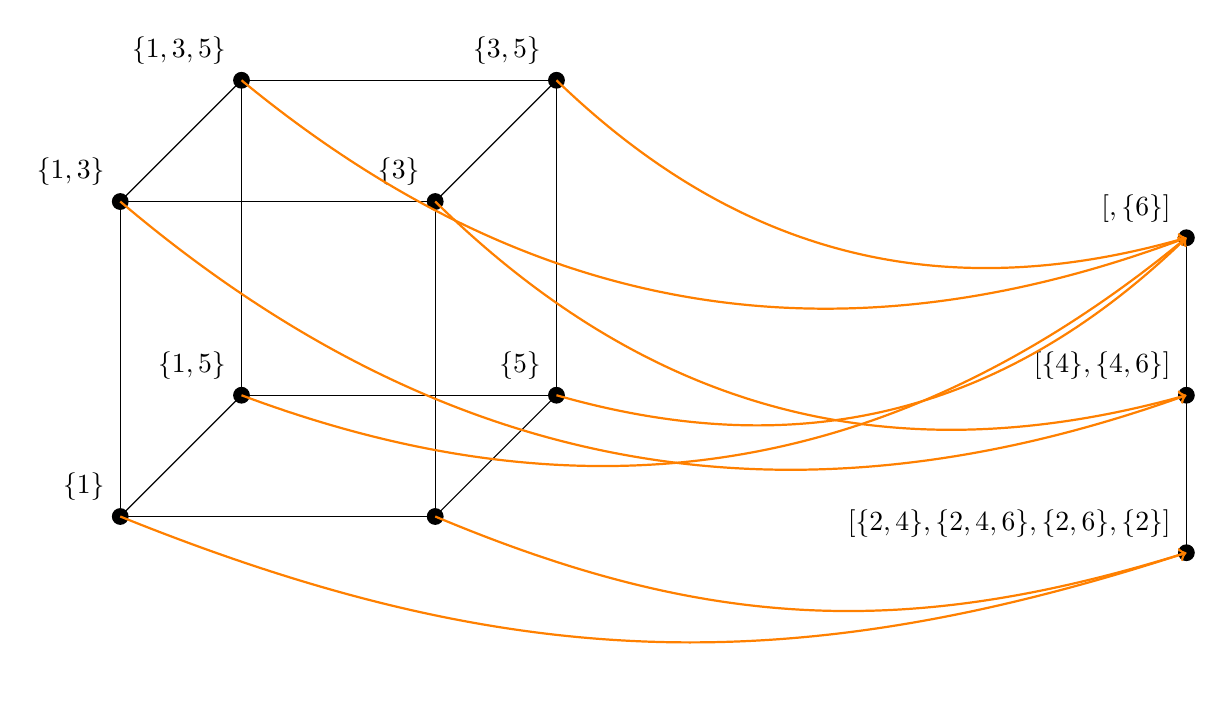
\begin{tikzpicture}[transform shape]

        \coordinate (A) at (0,0,0);
        \coordinate (B) at (4,0,0);
        \coordinate (C) at (4,4,0);
        \coordinate (D) at (0,4,0);
        \coordinate (E) at (0,0,4);
        \coordinate (F) at (4,0,4);
        \coordinate (G) at (4,4,4);
        \coordinate (H) at (0,4,4);

        \foreach \p/\t in { A/{$\{1,5\}$},
                            B/{$\{5\}$},
                            C/{$\{3,5\}$},
                            D/{$\{1,3,5\}$},
                            E/{\{1\}},
                            F/{$\varnothing$},
                            G/{$\{3\}$},
                            H/{$\{1,3\}$}}
            \node[draw, fill, circle, inner sep=2pt, label={135:\t}] (A\p) at (\p) {};

        \draw (A) -- (B) -- (C) -- (D) -- cycle; % Base
        \draw (E) -- (F) -- (G) -- (H) -- cycle; % Top
        \draw (A) -- (E);
        \draw (B) -- (F);
        \draw (C) -- (G);
        \draw (D) -- (H);

        %retta 
        \coordinate (J) at (12,0,0);
        \coordinate (K) at (12,2,0);
        \coordinate (N) at (12,-2,0);

        %connetto i punti
        \draw (J) -- (K) -- (N); 


        \foreach \p/\t in { J/{$[\{4\},\{4,6\}]$},
                            K/{$[\varnothing,\{6\}]$},
                            N/{$[\{2,4\},\{2,4,6\},\{2,6\},\{2\}]$}}
            \node[draw, fill, circle, inner sep=2pt, label={135:\t}] (B\p) at (\p) {};

            \draw[->, color=orange, bend right=20, thick] (E) to node[above] {} (N);
            \draw[->, color=orange, bend right=20, thick] (F) to node[above] {} (N);
            \draw[->, color=orange, bend right=30, thick] (G) to node[above] {} (J);
            \draw[->, color=orange, bend right=30, thick] (H) to node[above] {} (J);
            \draw[->, color=orange, bend right=30, thick] (A) to node[above] {} (K);
            \draw[->, color=orange, bend right=30, thick] (B) to node[above] {} (K);
            \draw[->, color=orange, bend right=30, thick] (C) to node[above] {} (K);
            \draw[->, color=orange, bend right=30, thick] (D) to node[above] {} (K);
\end{tikzpicture}
\end{figure}
Definiamo quindi una relazione di equivalenza tale per cui, se prendiamo 
anziché gli elementi astratti, le classi di equivalenza rispetto a tale relazione,
otteniamo un'inserzione di Galois, senza variare le funzioni 
$\alpha$ e $\gamma$, riducendo il dominio astratto.

Vediamo come questi formalismi (\textit{in particolare l'inserzione di
Galois}) sono equivalenti ad altri due formalismi, che però spostano 
l'osservazione dal dominio astratto, ovvero $\mathcal{A}$,
che ha una propria rappresentazione, a quello del dominio degli oggetti 
concreti che vogliamo osservare. Invece di guardare un mondo astratto 
rappresentato in un modo diverso, osserviamo il loro significato sul 
mondo concreto. Specifichiamo gli oggetti che osserviamo con precisione, ma 
nel mondo concreto e quindi modello con una funzione, chiamata \textbf{
funzione di chiusura superiore}, o un sottodominio, chiamato 
\textbf{Moore family}, ovvero l'astrazione del dominio concreto.

\section{Operatore di chiusura superiore (\texttt{UCO})}
Introduciamo questo nuovo concetto, che è una tipologia di funzioni che possiamo 
definire su un dominio. Supponiamo di avere un dominio $\mathcal{P}$ con un suo 
ordinamento $\leq_\mathcal{P}$ (\textit{in generale su reticoli completi}).

Allora una funzione $\rho : \mathcal{P} \to \mathcal{P}$ è un \texttt{UCO} 
se la funzione $\rho$ è:
\begin{itemize}
    \item \textbf{Monotona}: $\forall x,y \in \mathcal{P} \quad x \leq_\mathcal{P} y \implies \rho(x) \leq_\mathcal{P} \rho(y)$;
    \item \textbf{Estensiva}: $\forall x \in \mathcal{P} \quad x \leq_\mathcal{P} \rho(x)$;
    \item \textbf{Idempotente}: $\forall x \in \mathcal{P} \quad \rho(\rho(x)) = \rho(x)$.
\end{itemize}
Ovvero che $\rho$ può perdere informazione, ma tale informazione viene persa 
tutta in un'unica applicazione, ogni successiva applicazione non aggiunge
ulteriore imprecisione.

\begin{tcolorbox}[title = $\gamma \circ \alpha$ è un \texttt{UCO} nelle connessioni di Galois]
Questo perché sappiamo che $\gamma \circ \alpha$ è monotona, poiché 
si tratta di composizione di funzioni monotone, è estensiva perché
nelle proprietà delle connessioni di Galois abbiamo che 
$\gamma \circ \alpha(c) \geq c$ ed è idempotente, ovvero
perché $\gamma \circ \alpha \circ \gamma \circ \alpha(c) = 
\gamma \circ \texttt{id} \circ \alpha(c) = \gamma \circ \alpha(c)$, poiché 
$\gamma \circ \alpha \equiv \texttt{id}$.  
\end{tcolorbox}
